\section{UML Design} \label{section_classes}

The UML Diagram for the web application is depicted in the figure \ref{fig:webapp_class_diagram} below.
The diagram presents an extension of the \textbf{Model-View-Controller} architecture pattern. \\ \\

\vspace{20mm}

\begin{figure}[ht]
	\centering
	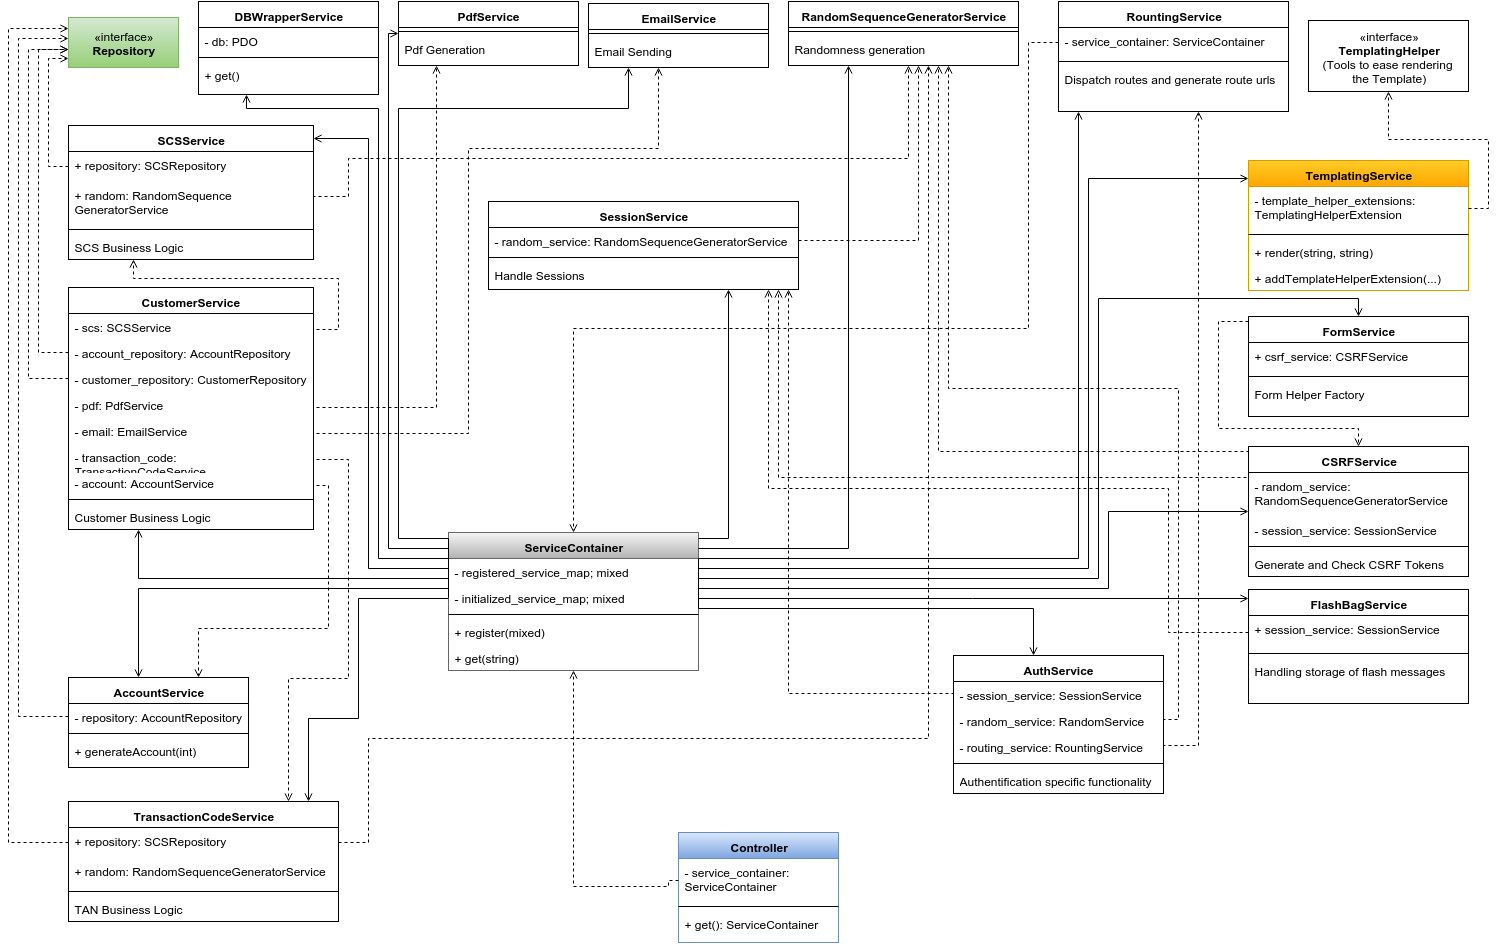
\includegraphics[width=0.9\linewidth]{figures/webapp_class_diagram.png}
	\caption{UML Diagram for the SecureBank application}
	\label{fig:webapp_class_diagram}
\end{figure}

\clearpage

The main categories of classes in the application are: 
\begin{itemize}
\item \textbf{Controller} - These classes are responsible for all operations concerning the working. \textit{Example: CustomerController handles all customer-related functionalities}. A main Controller is defined and all other controllers inherit from the base controller, adding additional and specific functionality.

\item \textbf{Model} - These classes represent the format of specific data objects. Example: \textit{Customer Model} defines the structure of a Customer object.

\item \textbf{Repository} - These classes handle the interaction with the database and contain the queries. Similar to the case of controllers, a base Repository is defined and all other repositories inherit from it.

All common functionality such as \textit{add}, \textit{update}, \textit{get} and \textit{find} are implemented in the base repository. So queries for these operations for any tables, need not be explicitly written. Rather, the functions need to be merely  invoked with the required parameters.
Extensive queries such as \textbf{JOINS} are written in the respective repositories, as per requirement.

\item \textbf{Service} - The \textit{Service} classes offer common functionality to be used across various other classes. Examples include \textit{CSRFService}, \textit{SessionService}, \textit{EmailService}, \textit{PdfService}, \textit{RandomSequenceGeneratorService} etc.

\item \textbf{Template} - \textit{Template} represents the \textbf{View}. So all templates are files containing HTML code, to be rendered on the web. Adhering to good coding practices, all client-side scripting is kept out of the HTML and handled separately in a JavaScript file.

\end{itemize}

\clearpage